\documentclass{article}
\usepackage[russian]{babel}
\usepackage{amsfonts}
\usepackage{graphicx}
\usepackage{mathtools}
\usepackage[T1]{fontenc}
\usepackage[export]{adjustbox}
\graphicspath{{pictures/}}
\DeclareGraphicsExtensions{.pdf,.png,.jpg}
\usepackage{amsthm}
\usepackage[14pt]{extsizes}
\vspace{50mm}
\setlength{\parskip}{1.2em}
\linespread{1.2}
\usepackage[left=25mm, top=25mm, right=25mm, bottom=25mm, nohead]{geometry}
\newtheorem{theorem}{Утверждение}

\begin{document}
\thispagestyle{empty}
\begin{center}
\large \textbf{МИНОБРНАУКИ РОССИИ}\\
\normalsize{федеральное государственное бюджетное образовательное\\
учреждение высшего образования}\\
\large \textbf{Национальный исследовательский университет «МЭИ»}\\
\noindent\rule{15cm}{0.4pt}
\end{center}
\begin{flushright}
\large \textbf {Институт \underline {ИВТИ}}\\
\large \textbf {Кафедра \underline {ПМИИ}}\\
\end{flushright}
\begin{center}
\large \textbf{Теоритические модели вычислений}\\
\large{ДЗ №1: Регулярные языки и конечныеавтоматы}\\
\end{center}
\hfill \break
\begin{flushright}
{Выполнил: студент группы А-13а-19 
\\Тулинов А.В.\\
Преподаватель: Ивлиев С. А.}\\
\end{flushright}
\hfill \break
\hfill \break
\hfill \break
\begin{center}
Москва, 2022 г.
\end{center}

\newpage
\textbf{\Large Задание №1. Построить конечный автомат, распознающий язык (5 баллов)}\\
\hfill \break
\normalsize{Ответом на данное задание является конечный автомат, распознающий описанный язык. Автомат должен быть детерминированным.}\\
\hfill \break
1. \(L = \{\omega  \in \{a,b,c\}^* \mid |\omega|_c = 1\}\) (1 балл)\\
\hfill \break
\normalsize{Построенный автомат распознает язык, в котором обязательно будет присутствовать ровно одна буква c.}\\
\includegraphics [scale=0.4]{task1_1}
\hfill \break
2. \(L = \{\omega  \in \{a,b\}^* \mid |\omega|_a \leq 2, |\omega|_b \geq 2\}\) (1 балл)\\
\(L_1 = \{\omega  \in \{a,b\}^* \mid |\omega|_a \leq 2\}\)\\
\(L_2 = \{\omega  \in \{a,b\}^* \mid |\omega|_b \geq 2\}\)
\begin{figure} [h]
\center{\includegraphics[scale=0.5]{task1_2_tmp}}
\caption{Автомат распознает язык \(L_1\)}
\end{figure}
\begin{figure}[h]
\center{\includegraphics[scale=0.5]{task1_2_tmp_1}}
\caption{Автомат распознает язык \(L_2\)}
\end{figure}
\hfill \break
\normalsize{Построим прямое произведение двух ДКА:}\\
\(\Sigma = \{a,b\}\)\\
\(Q = \{(q_1,q_4), (q_1,q_5),(q_1,q_6),(q_2,q_4),(q_2,q_5),(q_2,q_6),(q_3,q_4),(q_3,q_5),(q_3,q_6)\}\)\\
\(S = \{q_1,q_4\}\)\\
\(T = \{(q_1,q_6),(q_2,q_6),(q_3,q_6)\}\)
\begin{center}
\begin{tabular} {|c |c |c|}
\hline
\multicolumn{3}{|c|}{Таблица переходов ДКА} \\
\hline
 & a & b \\
\hline
\(q_1,q_4\) & \(q_2,q_4\) & \(q_1,q_5\) \\
\hline
\(q_1,q_5\) & \(q_2,q_5\) & \(q_1,q_6\) \\
\hline
\(q_1,q_6\) & \(q_2,q_6\) & \(q_1,q_6\) \\
\hline
\(q_2,q_4\) & \(q_3,q_4\) & \(q_2,q_5\) \\
\hline
\(q_2,q_5\) & \(q_3,q_5\) & \(q_2,q_6\) \\
\hline
\(q_2,q_6\) & \(q_3,q_6\) & \(q_2,q_6\) \\
\hline
\(q_3,q_4\) & \(\emptyset\) & \(q_3,q_5\) \\
\hline
\(q_3,q_5\) & \(\emptyset\) & \(q_3,q_6\) \\
\hline
\(q_3,q_6\) & \(\emptyset\) & \(q_3,q_6\) \\
\hline
\end{tabular}
\end{center}
\normalsize{Автомат распознающий заданный язык L: }\\
\hfill \break
\includegraphics [scale=0.7]{task1_2}\\
\hfill \break
\hfill \break
3. \(L = \{\omega  \in \{a,b\}^* \mid |\omega|_a \neq |\omega|_b\}^*\) (1 балл)\\
\hfill \break
\normalsize{Нельзя построить автомат, потому что необходимо запомнинать количество символов.}\\
\hfill \break
4. \(L = \{\omega  \in \{a,b\}^* \mid \omega \omega = \omega \omega \omega \}\) (2 балла)\\
\hfill \break
\normalsize{Построенный автомат распознает язык, состоящий из пустого слова.}\\
\hfill \break
\includegraphics {task1_4}\\
\hfill \break
\newpage

\textbf{\Large Задание №2. Построить конечный автомат, используя прямое произведение  (5 баллов)}\\
\hfill \break
\normalsize{Ответом на данное задание является конечный автомат, распознающий описанный язык. Требуется, чтобы он был построен при помощи прямого произведения ДКА и его свойств.}\\
\hfill \break
1. \(L_1 = \{\omega  \in \{a,b\}^* \mid |\omega|_a \geq 2  \land |\omega|_b \geq 2\}\) (1 балл)\\
\hfill \break
\(L_1' = \{\omega  \in \{a,b\}^* \mid |\omega|_a \geq 2\}\)\\
\(L_2' = \{\omega  \in \{a,b\}^* \mid |\omega|_b \geq 2\}\)\\
\hfill \break
\begin{figure}[h]
\center{\includegraphics[scale=0.6]{task2_1_tmp}}
\caption{Автомат распознает язык \(L_1'\)}
\end{figure}
\begin{figure}[h]
\center{\includegraphics[scale=0.6]{task1_2_tmp_1}}
\caption{Автомат распознает язык \(L_2'\)}
\end{figure}
\hfill \break
\normalsize{Построим прямое произведение двух ДКА:}\\
\(\Sigma = \{a,b\}\)\\
\(Q = \{(q_1,q_4), (q_1,q_5),(q_1,q_6),(q_2,q_4),(q_2,q_5),(q_2,q_6),(q_3,q_4),(q_3,q_5),(q_3,q_6)\}\)\\
\(S = \{q_1,q_4\}\)\\
\(T = \{q_3,q_6\}\)\\
\begin{center}
\begin{tabular} {|c |c |c|}
\hline
\multicolumn{3}{|c|}{Таблица переходов ДКА} \\
\hline
 & a & b \\
\hline
\(q_1,q_4\) & \(q_2,q_4\) & \(q_1,q_5\) \\
\hline
\(q_1,q_5\) & \(q_2,q_5\) & \(q_1,q_6\) \\
\hline
\(q_1,q_6\) & \(q_2,q_6\) & \(q_1,q_6\) \\
\hline
\(q_2,q_4\) & \(q_3,q_4\) & \(q_2,q_5\) \\
\hline
\(q_2,q_5\) & \(q_3,q_5\) & \(q_2,q_6\) \\
\hline
\(q_2,q_6\) & \(q_3,q_6\) & \(q_2,q_6\) \\
\hline
\(q_3,q_4\) & \(q_3,q_4\) & \(q_3,q_5\) \\
\hline
\(q_3,q_5\) & \(q_3,q_5\) & \(q_3,q_6\) \\
\hline
\(q_3,q_6\) & \(q_3,q_6\) & \(q_3,q_6\) \\
\hline
\end{tabular}
\end{center}
\normalsize{Автомат распознающий заданный язык \(L_1\): }\\
\includegraphics [scale=0.8]{task2_1}\\
\hfill \break
\hfill \break
\hfill \break
2. \(L_2 = \{\omega  \in \{a,b\}^* \mid |\omega| \geq 3 \land |\omega| \text{ нечётное}\}\) (1 балл)\\
\hfill \break
\(L_1' = \{\omega  \in \{a,b\}^* \mid |\omega| \geq 3\}\)\\
\(L_2' = \{\omega  \in \{a,b\}^* \mid |\omega| \text{ нечётное}\}\)\\
\begin{figure}[h]
\center{\includegraphics[scale=0.7]{task2_2_tmp}}
\caption{Автомат распознает язык \(L_1'\)}
\end{figure}
\hfill \break
\begin{figure}[h]
\center{\includegraphics[scale=0.7]{task2_2_tmp_1}}
\caption{Автомат распознает язык \(L_2'\)}
\end{figure}
\hfill \break
\normalsize{Построим прямое произведение двух ДКА:}\\
\(\Sigma = \{a,b\}\)\\
\(Q = \{(q_1,q_5), (q_1,q_6),(q_2,q_5),(q_2,q_6),(q_3,q_5),(q_3,q_6),(q_4,q_5),(q_4,q_6)\}\)\\
\(S = \{q_1,q_5\}\)\\
\(T = \{q_4,q_6\}\)\\
\begin{center}
\begin{tabular} {|c |c |c|}
\hline
\multicolumn{3}{|c|}{Таблица переходов ДКА} \\
\hline
 & a & b \\
\hline
\(q_1,q_5\) & \(q_2,q_6\) & \(q_2,q_6\) \\
\hline
\(q_1,q_6\) & \(q_2,q_5\) & \(q_2,q_5\) \\
\hline
\(q_2,q_5\) & \(q_3,q_6\) & \(q_3,q_6\) \\
\hline
\(q_2,q_6\) & \(q_3,q_5\) & \(q_3,q_5\) \\
\hline
\(q_3,q_5\) & \(q_4,q_6\) & \(q_4,q_6\) \\
\hline
\(q_3,q_6\) & \(q_4,q_5\) & \(q_4,q_5\) \\
\hline
\(q_4,q_5\) & \(q_4,q_6\) & \(q_4,q_6\) \\
\hline
\(q_4,q_6\) & \(q_4,q_5\) & \(q_4,q_5\) \\
\hline
\end{tabular}
\end{center}
\normalsize{Автомат распознающий заданный язык \(L_2\): }\\\\
\includegraphics [scale=0.6]{task2_2}\\
\hfill \break
\normalsize{Полученный результат можно упростить:}\\
\hfill \break
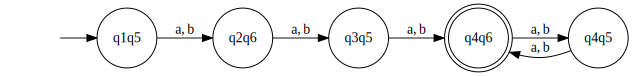
\includegraphics [scale=0.8]{task2_2_simple}\\\\\\
\hfill \break
\hfill \break
\hfill \break
\hfill \break
\hfill \break
3. \(L_3 = \{\omega  \in \{a,b\}^* \mid |\omega|_a \text{ чётно} \land |\omega|_b \text{ кратно трём} \}\) (1 балл)\\
\hfill \break
\(L_1' = \{\omega  \in \{a,b\}^* \mid |\omega|_a \text{ чётно}\}\)\\
\(L_2' = \{\omega  \in \{a,b\}^* \mid |\omega|_b \text{ кратно трём}\}\)\\
\begin{figure}[h]
\center{\includegraphics[scale=0.7]{task2_3_tmp}}
\caption{Автомат распознает язык \(L_1'\)}
\end{figure}
\begin{figure}[h]
\center{\includegraphics[scale=0.7]{task2_3_tmp_1}}
\caption{Автомат распознает язык \(L_2'\)}
\end{figure}
\hfill \break
\normalsize{Построим прямое произведение двух ДКА:}\\
\(\Sigma = \{a,b\}\)\\
\(Q = \{(q_1,q_3), (q_1,q_4),(q_1,q_5),(q_2,q_3),(q_2,q_4),(q_2,q_5)\}\)\\
\(S = \{q_1,q_3\}\)\\
\(T = \{q_1,q_3\}\)\\
\begin{center}
\begin{tabular} {|c |c |c|}
\hline
\multicolumn{3}{|c|}{Таблица переходов ДКА} \\
\hline
 & a & b \\
\hline
\(q_1,q_3\) & \(q_2,q_3\) & \(q_1,q_4\) \\
\hline
\(q_1,q_4\) & \(q_2,q_4\) & \(q_1,q_5\) \\
\hline
\(q_1,q_5\) & \(q_2,q_5\) & \(q_1,q_3\) \\
\hline
\(q_2,q_3\) & \(q_1,q_3\) & \(q_2,q_4\) \\
\hline
\(q_2,q_4\) & \(q_1,q_4\) & \(q_2,q_5\) \\
\hline
\(q_2,q_5\) & \(q_1,q_5\) & \(q_2,q_3\) \\
\hline
\end{tabular}
\end{center}
\normalsize{Автомат распознающий заданный язык \(L_3\): }\\\\
\includegraphics [scale=0.7]{task2_3}\\
\hfill \break
4. \(L_4 = \bar{L_3}\) (1 балл)\\
\hfill \break
\normalsize{Для того чтобы получить отрицание,  нужно инвертировать все терминальные и нетерминальные вершины у автомата, распознающего язык \(L_3\).}\\
\normalsize{Автомат распознающий заданный язык \(L_4\): }\\\\
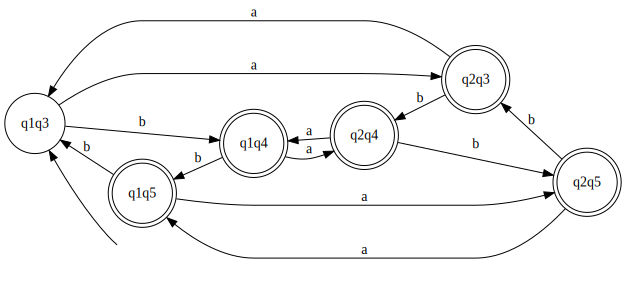
\includegraphics [scale=0.7]{task2_4}\\
\hfill \break
5. \(L_5 = L_2 \backslash L_3\) (1 балл)\\
\hfill \break
 \(L_5 = L_2 \backslash L_3\ = L_2 \cap \bar{L_3} =  L_2 \cap L_4\)\\
\normalsize{Поменяем нуммерацию для \(L_4\): }\\
\includegraphics {task2_4_simple}\\
\normalsize{Поменяем нуммерацию для \(L_2\): }\\
\includegraphics [scale=0.7]{task2_2_super_simple}\\
\normalsize{Построим прямое произведение двух ДКА:}\\
\(\Sigma = \{a,b\}\)\\
\(Q = \{(1,7),(1,8),(1,9),(1,10),\\
(2,7),(2,8),(2,9),(2,10),\\
(3,7),(3,8),(3,9),(3,10),\\
(4,7),(4,8),(4,9),(4,10),\\
(5,7),(5,8),(5,9),(5,10),\\
(6,7),(6,8),(6,9),(6,10)\}\)\\
\(S = \{1,7\}\)\\
\(T = \{(2,10),(3,10),(4,10),(5,10),(6,10)\}\)\\

\begin{center}
\begin{tabular} {|c |c |c|}
\hline
\multicolumn{3}{|c|}{Таблица переходов ДКА} \\
\hline
 & a & b \\
\hline
(1,7) & (4,8) & (2,8) \\
\hline
(1,8) & (4,9) & (2,9) \\
\hline
(1,9) & (4,10) & (2,10) \\
\hline
(1,10) & (4,9) & (2,9) \\
\hline
\hline
(2,7) & (5,8) & (3,8) \\
\hline
(2,8) & (5,9) & (3,9) \\
\hline
(2,9) & (5,10) & (3,10) \\
\hline
(2,10) & (5,9) & (3,9) \\
\hline
\hline
(3,7) & (6,8) & (1,8) \\
\hline
(3,8) & (6,9) & (1,9) \\
\hline
(3,9) & (6,10) & (1,10) \\
\hline
(3,10) & (6,9) & (1,9) \\
\hline
\hline
(4,7) & (1,8) & (5,8) \\
\hline
(4,8) & (1,9) & (5,9) \\
\hline
(4,9) & (1,10) & (5,10) \\
\hline
(4,10) & (1,9) & (5,9) \\
\hline
\hline
(5,7) & (2,8) & (6,8) \\
\hline
(5,8) & (2,9) & (6,9) \\
\hline
(5,9) & (2,10) & (6,10) \\
\hline
(5,10) & (2,9) & (6,9) \\
\hline
\hline
(6,7) & (3,8) & (4,8) \\
\hline
(6,8) & (3,9) & (4,9) \\
\hline
(6,9) & (3,10) & (4,10) \\
\hline
(6,10) & (3,9) & (4,9) \\
\hline
\end{tabular}
\end{center}
\normalsize{Автомат распознающий заданный язык \(L_5\): }\\\\
\includegraphics [scale=0.5]{task2_5}\\
\hfill \break
\normalsize{Полученный результат можно упростить:}\\
\hfill \break
\includegraphics [scale=0.5]{task2_5_simple}\\

\newpage
\textbf{\Large Задание №3. Построить минимальный ДКА, по регулярному выражению (5 баллов)}\\
\hfill \break
\normalsize{Ответом на данное задание является минимальный ДКА, который допускает тот же язык, что описывается регулярным выражением.}\\
\hfill \break
1. \((ab + aba)^*a\) (1 балл)\\
\hfill \break
\normalsize{Построим  НКА}\\
\hfill \break
\includegraphics [scale=0.7]{task3_1_nka}\\
\begin{center}
\begin{tabular} {|c |c |c|}
\hline
 & a & b \\
\hline
\(q_1\) & \(q_2q_3q_4\) & \(\) \\
\hline
\(q_2q_3q_4\) & \(\) & \(q_1q_5\) \\
\hline
\(q_1q_5\) & \(q_1q_2q_3q_4\) & \(\) \\
\hline
\(q_1q_2q_3q_4\) & \(q_2q_3q_4\) & \(q_1q_5\) \\
\hline
\end{tabular}
\end{center}
\normalsize{Построим  ДКА}\\
\includegraphics [scale=0.8]{task3_1_dka}\\
\hfill \break
2. \(a(a(ab)^*b)^*(ab)^*\) (1 балл)\\
\hfill \break
\hfill \break
\includegraphics [scale=0.8]{task3_2_nka}\\
\normalsize{Преобразуем:}\\
\hfill \break
\includegraphics [scale=0.8]{task3_2_dka}\\
\hfill \break
3. \((a + (a + b)(a + b)b)^*\) (1 балл)\\
\hfill \break
\normalsize{Построим  НКА}\\
\hfill \break
\includegraphics {task3_3_nka}\\
\hfill \break
\begin{center}
\begin{tabular} {|c |c |c|}
\hline
 & a & b \\
\hline
\(q_1\) & \(q_1q_2\) & \(q_2\) \\
\hline
\(q_1q_2\) & \(q_1q_2q_3\) & \(q_2q_3\) \\
\hline
\(q_2\) & \(q_3\) & \(q_3\) \\
\hline
\(q_1q_2q_3\) & \(q_1q_2q_3\) & \(q_1q_2q_3\) \\
\hline
\(q_2q_3\) & \(q_3\) & \(q_1q_3\) \\
\hline
\(q_3\) & \(\) & \(q_1\) \\
\hline
\(q_1q_3\) & \(q_1q_2\) & \(q_1q_2\) \\
\hline
\end{tabular}
\end{center}
\normalsize{Построим  ДКА}\\
\hfill \break
\includegraphics[scale=0.8] {task3_3_dka}\\
\hfill \break
4. \((b + c)((ab)^*c + (ba)^*)^*\) (1 балл)\\
\hfill \break
\normalsize{Построим  ДКА}\\
\hfill \break
\includegraphics[scale=0.8] {task3_4_dka}\\
\hfill \break
5. \((a+b)^+(aa+bb+abab+baba)(a+b)^+\) (1 балл)\\
\hfill \break
\normalsize{Построим  НКА}\\
\hfill \break
\includegraphics[scale = 0.7] {task3_5_nka}\\
\hfill \break
\begin{center}
\begin{tabular} {|c |c |c|}
\hline
 & a & b \\
\hline
\(q_1\) & \(q_2\) & \(q_2\) \\
\hline
\(q_2\) & \(q_2q_3\) & \(q_2q_7\) \\
\hline
\(q_2q_3\) & \(q_2q_3q_6\) & \(q_2q_4q_7\) \\
\hline
\(q_2q_7\) & \(q_2q_3q_8\) & \(q_2q_6q_7\) \\
\hline
\(q_2q_3q_6\) & \(q_2q_3q_6q_{10}\) & \(q_2q_6q_7q_{10}\) \\
\hline
\(q_2q_4q_7\) & \(q_2q_3q_5q_8\) & \(q_2q_6q_7\) \\
\hline
\(q_2q_3q_8\) & \(q_2q_3q_6\) & \(q_2q_4q_7q_9\) \\
\hline
\(q_2q_6q_7\) & \(q_2q_3q_8q_{10}\) & \(q_2q_6q_7q_{10}\) \\
\hline
\(q_2q_3q_6q_{10}\) & \(q_2q_3q_6q_{10}\) & \(q_2q_4q_7q_{10}\) \\
\hline
\(q_2q_6q_7q_{10}\) & \(q_2q_3q_8q_{10}\) & \(q_2q_6q_7q_{10}\) \\
\hline
\(q_2q_3q_5q_8\) & \(q_2q_3q_6\) & \(q_2q_4q_6q_7q_9\) \\
\hline
\(q_2q_4q_7q_9\) & \(q_2q_3q_5q_6q_8\) & \(q_2q_6q_7\) \\
\hline
\(q_2q_3q_8q_{10}\) & \(q_2q_3q_6q_{10}\) & \(q_2q_4q_7q_9q_{10}\) \\
\hline
\(q_2q_4q_7q_{10}\) & \(q_2q_3q_5q_8q_{10}\) & \(q_2q_6q_7q_{10}\) \\
\hline
\(q_2q_3q_5q_8q_{10}\) & \(q_2q_3q_6q_{10}\) & \(q_2q_4q_6q_7q_9q_{10}\) \\
\hline
\(q_2q_4q_6q_7q_9\) & \(q_2q_3q_5q_6q_8q_{10}\) & \(q_2q_6q_7q_{10}\) \\
\hline
\(q_2q_3q_5q_6q_8\) & \(q_2q_3q_6q_{10}\) & \(q_2q_4q_6q_7q_9q_{10}\) \\
\hline
\(q_2q_4q_7q_9q_{10}\) & \(q_2q_3q_5q_6q_8q_{10}\) & \(q_2q_6q_7q_{10}\) \\
\hline
\(q_2q_4q_6q_7q_9q_{10}\) & \(q_2q_3q_5q_6q_8q_{10}\) & \(q_2q_6q_7q_{10}\) \\
\hline
\(q_2q_3q_5q_6q_8q_{10}\) & \(q_2q_3q_6q_{10}\) & \(q_2q_4q_6q_7q_9q_{10}\) \\
\hline
\end{tabular}
\end{center}
\hfill \break
\normalsize{Построим  ДКА}\\
\includegraphics[scale = 0.2] {task3_5_dka}\\

\newpage
\textbf{\Large Задание №4. Определить является ли язык регулярным или нет (5 баллов)}\\
\hfill \break
\normalsize{Ответом на данное задание является конечный автомат, если язык регу-
лярен, либо доказательство нерегулярности языка при помощи леммы о разрастании.}\\
\hfill \break
1. \(L = \{(aab)^nb(aba)^m  \mid n \geq 0, m \geq 0\}\) (1 балл)\\
\hfill \break
\includegraphics {task4_1}\\
2. \(L = \{uaav \mid u \in \{a,b\}^*, v \in \{a, b\}^*, |u|_b \geq |v|_a\}\) (1 балл)\\
\hfill \break
\normalsize \textbf{Язык не является регулярным.}\\\\
Пусть \( \bar{L} = \{uaav \mid u \in \{a,b\}^*, v \in \{a, b\}^*, |u|_b < |v|_a \}\)\\
Зафиксируем n.\\
Пусть \( w = b^naaa^{n+1} \in  \bar{L}; |w| \geq n.\) (Разбиения при \(|xy| \leq n, |y| \geq 1\))\\
 \(w = xyz\)\\
 \( x = b^l\)\\
 \( y = b^k\)\\
 \( z = b^{n-l-k}aaa^{n+1}\)\\
{При накачке y, количество символов b превысит количество символов а} \(\Rightarrow w \notin \bar{L} \Rightarrow \bar{L} - \text{нерегулярный} \Rightarrow L - \text{нерегулярный.}\)\\
\hfill \break
3. \(L = \{a^m\omega \mid \omega \in \{a,b\}^*, 1 \leq  |\omega|_b \leq m\}\) (1 балл)\\
\hfill \break
\normalsize \textbf{Язык не является регулярным.}\\\\
Пусть \( \bar{L} = \{a^m\omega \mid \omega \in \{a,b\}^*, |\omega|_b > m \vee  |\omega|_b = 0\}\)\\
Зафиксируем n.\\
Пусть \( w = a^nb^{n+1} \in  \bar{L}; |w| \geq n.\) (Разбиения при \(|xy| \leq n, |y| \geq 1\))\\
 \(w = xyz\)\\
 \( x = a^l\)\\
 \( y = a^k\)\\
 \( z = a^{n-l-k}b^{n+1}\)\\
{При накачке y, количество символов a превысит количество символов b} \(\Rightarrow w \notin \bar{L} \Rightarrow \bar{L} - \text{нерегулярный} \Rightarrow L - \text{нерегулярный.}\)\\\\
4. \(L = \{a^kb^ma^n \mid k = n \lor m > 0 \}\) (1 балл)\\
\hfill \break
\normalsize \textbf{Язык не является регулярным.}\\\\
Зафиксируем n.\\
Пусть \( w = a^nba^n; |w| \geq n.\)\\
 \(w = xyz\)\\
 \( x = a^l\)\\
 \( y = a^k\)\\
 \( z = a^{n-l-k}ba^n\)\\
{При накачке y, условие k = n - не выполняется} \(\Rightarrow w \notin L \Rightarrow L - \text{нерегулярный.}\)\\\\
\hfill \break
5. \(L = \{ucv \mid u \in \{a,b\}^*, v \in \{a,b\}^*, u \neq v^R\}\) (1 балл)\\
\hfill \break
\normalsize \textbf{Язык не является регулярным.}\\\\
Пусть \( \bar{L} =  \{ucv \mid u \in \{a,b\}^*, v \in \{a,b\}^*, u = v^R\}\)\\
Зафиксируем n.\\
Пусть \( w = a^nca^{n} \in  \bar{L}; |w| \geq n.\) (Разбиения при \(|xy| \leq n, |y| \geq 1\))\\
 \(w = xyz\)\\
 \( x = a^l\)\\
 \( y = a^k\)\\
 \( z = a^{n-l-k}ca^{n}\)\\
Очевидно, что при накачке y условие \( u = v^R - \) не выполняется \(\Rightarrow w \notin \bar{L} \Rightarrow \bar{L} - \text{нерегулярный} \Rightarrow L - \text{нерегулярный.}\)
\newpage
\textbf{\Large Задание №5. Реализовать алгоритмы (10 баллов)}\\
\hfill \break
\normalsize{Ответом на данное задание является работающая программа на выбранном
языке программирования, покрытая юнит-тестами.}\\
\hfill \break
\normalsize{В рамках своего выполнения программа должна генерировать текстовый
документ с картинками, показывающий процесс построения автомата (к
примеру Markdown с графиками на Graphviz).}\\
\hfill \break
\normalsize{ 1. Построение ДКА по НКА с \(\lambda\)-переходами } (5 баллов)\\
\hfill \break
\normalsize{2. Прямое произведение языков, с возможностью построить пересечение,
объединение и разность} (5 баллов)\\
\hfill \break
\end{document}
